% Auth: Simon Symeonidis
% -----------------------------------

\documentclass[twoside]{article}

\title{A Case Study in Ada2012: Implementing a simple Http Server}

\author{Simon J. Symeonidis}

\date{\today}

\usepackage[margin=0.8in]{geometry}
\usepackage{fancyhdr}
\usepackage{float}
\usepackage{url}
\usepackage{ulem}
\usepackage[pdftex]{graphicx}
\usepackage{listings}
\usepackage{titlesec}
\usepackage{titletoc}
\usepackage{xcolor}
% \usepackage{savetrees}
\usepackage{cite}

% COLOR DEFINITIONS
\definecolor{blue}{RGB}{0,0,255}
\definecolor{green}{RGB}{0,100,0}
\definecolor{psyan}{RGB}{0,104,222}
\definecolor{lightpsyan}{RGB}{185,239,254}
% END COLOR DEFS

\lstset{
xleftmargin=15pt,
linewidth=15cm,
framexleftmargin=5mm, 
frame=trBL, 
frameround=tftf,
basicstyle=\footnotesize,       % the size of the fonts that are used for the code
numbers=left,                   % where to put the line-numbers
numberstyle=\tiny,      % the size of the fonts that are used for the line-numbers
numbersep=5pt,                  % how far the line-numbers are from the code
identifierstyle=\ttfamily,
backgroundcolor=\color{white},  % choose the background color. You must add \usepackage{color}
keywordstyle=\color{blue},
commentstyle=\color{green},
showspaces=false,               % show spaces adding particular underscores
showstringspaces=false,         % underline spaces within strings
showtabs=false,                 % show tabs within strings adding particular underscores
tabsize=2,	                % sets default tabsize to 2 spaces
captionpos=b,                   % sets the caption-position to bottom
breaklines=true,                % sets automatic line breaking
breakatwhitespace=false        % sets if automatic breaks should only happen at whitespace
%%% colors
}

% Custom section style
\titleformat{\section}[frame]
{\color{psyan}\normalfont}
{\filleft \footnotesize ::Section \thesection ::}
{5pt}
{\Large\bfseries\filright}

% Paragraph indentation 
\setlength{\parindent}{0in}

\makeatletter
  \def\@seccntformat#1{\rlap{\hskip-36pt\csname the#1\endcsname}}
\makeatother


\renewcommand{\headrulewidth}{0pt}
\renewcommand{\footrulewidth}{0pt}


% subsections ...
% \titleformat*{\section}{\normalfont\Large\bfseries\color{psyan}}
% \titleformat*{\subsection}{\normalfont\large\bfseries\color{psyan}}
% \titleformat*{\subsubsection}{\normalfont\normalsize\bfseries\color{psyan}}

% paragraphs

% \titleformat*{\paragraph}{\normalfont\normalsize\bfseries\color{red}}
% \titleformat*{\subparagraph}{\normalfont\normalsize\bfseries\color{red}}

% TOC

%\renewcommand\thesection{\color{psyan}\arabic{section}}

\begin{document}

  \pagenumbering{roman}
  
  \pagestyle{fancy}
  \maketitle
  \newpage
  % \rhead[]{\textbf{\color{psyan}\nouppercase{\leftmark} \nouppercase{\rightmark}}}
  % \lhead[\textbf{\color{psyan}\nouppercase{\leftmark} \nouppercase{\rightmark}}]{}
  
  \newpage
  \setcounter{tocdepth}{5}
  \tableofcontents
  \listoffigures
  \lstlistoflistings
  \newpage
  
  \pagenumbering{arabic}
  
  \rfoot[]{\thepage}
  \cfoot{}
  \lfoot[\thepage]{}

  \section{Motivation} 
This is a small case study in the 2012 release of the Ada programming language. The motivation for this docuemnt and exercise is to introduce me to this technology, document my progress, and help others learn said language. The topic I have chosen is to write up a very simple web server. A web server typically, has to deal with the following aspects:
\begin{itemize}
\item Concurrency
\item Sockets, and messaging
\item Protocol implementation (in this case \textbf{http})
\item Different Filesystems support 
\end{itemize} 

These aspects go over a good set of small problems, that would expose uses of the language for multiple problem domains. 

\subsection{The name `Axios'}
Axios stands for ``Ada eXtra ineffectual Object Oriented Server''. And it is just that!
  \section{Topics of interest}
Here we discuss in a little more detail the previously outlined topics. These topics offer us a concise and detailed tests to investigate the the Ada 2012 progrqamming language, along with other tools that can be used to supplement and extend future projects. We will be looking at the following aspects:
\begin{itemize}
\item{The Ada2012} programming language (Language structure, strengths, weaknesses, etc)
\item{The Ada2012 Toolchain} The \textbf{gnat} compiler, the project manager files (gpr)
\item{AUnit} for a unit testing platform
\end{itemize}

\subsection{Concurrency}
Ada is considered to have a good concurrency support. 

% TODO Revise this part 
\subsection{Sockets}
Sockets are a good topic in this case study, since sockets are OS dependent
therefore will provide some insight on how the language and application will
behave on different platforms. 

\subsection{Cross Platform Filesystem Support}
To programmers that have used languages that do not require virtual machines, concerns for cross platform availability of an application, more often arise. This case study will use some simple filesystem operations to indicate what we may and may not do with the language. We will investigate how:
\begin{itemize}
  \item Location to resources are handled
  \item Permissions for inodes are handled
\end{itemize}

\subsection{Protocol Implementation}
A topic that I have came accross in programming languages that is somewhat
interesting to see in implementation, are protocols. Notably \textbf{Erlang} 
makes this a breeze. Investigating this in Ada will be interesting. 

For this small project, we'll be implementing 5 parts of the Http protocol. 
Namely the HEAD, GET, POST, PUT and DELETE methods. We refer to the RFC2616 manual \cite{RFC2616}
for the definition of behaviours of these methods. Once they are implemented in
this case study using Ada, the project shall be tested by using any mainstream 
browser such as \textit{Firefox} or \textit{Chromium}.

For the reader we extract the definitions and behaviour of these four methods.
\subsubsection{Overview of Http Protocol}
The Http protocol is a text, request-response protocol. The RFC2616 specification is quite detailed, but we will be implementing a very small subset of the specification for this case study.

The Http version we are concerned with is \textbf{1.1}. There exists indempodent and non indempodent methods in the Http specification. 

GET is described as an indempodent method. That is, if a request is being made with the same specific set of parameters, then the response should be the same each time that request is repeated. For example, if we had a function such as $ f(x) = x + 1 $, then each time we provided $ x = 1 $ we should always retrieve `2'. We present the following table, which describes the methods we will be implementing:
\\
\begin{center}
\begin{tabular}{| c | c |}
\hline
\textbf{Method} & \textbf{Type} \\ \hline \hline
HEAD   & Indempondent \\
GET    & Indempondent \\
POST   & Non-Indempondent \\
PUT    & Indempondent \\ 
DELETE & Indempondent \\
\hline
\end{tabular}
\end{center}
\subsubsection{HEAD}
This Http method requests the header fields of an html document. The message body is not to be retrieved. Here is an example of what http headers look like. The definition is taken straight out of the manual:  
\lstinputlisting[language=]{./src/misc/header-definition.txt}

Here is a more practical example. These headers are retrieved from \textit{www.google.ca}:
\lstinputlisting[language=]{./src/misc/html-header.txt}

And this is the expected html response definition from a successful request.
\lstinputlisting[language=]{./src/misc/http-response.txt}

\subsubsection{GET} 
A \textbf{GET} method is defined in the specification, to be used for operations that
require \textbf{reading} information. On the server side, this should not
tamper with the resources. 

A get request requires \textbf{Request-Line} field to be sent. It is up to the
server to look for the resource requested, and send the response afterwards.

Taken directly from the manual, here is a demonstration of what the GET request
looks like, when ``accessing www.w3.org'':
\lstinputlisting[language=]{./src/misc/get-request.txt}

\subsubsection{POST}
\textbf{POST} is the indempodent method we mentioned before. This means each
time a post request is sent, a resource must (usually) be created, always
guaranteeing different response, for a same request.

A more ``hands on'' example of this would be if a user accidentally submited a
form twice by an accidental double click.

\subsubsection{PUT}
We must add more stuff here.

\subsubsection{DELETE} 
We must add more stuff here.

\subsection{First Steps}
The first steps in an Ada application is to define the \textit{project manager 
file} for the given project as outlined on the manual \cite{GNATintro}.

%% TODO: Need to check if this is indeed the case. 
The GNAT project file abstracts a lot of the building details into this file. It will take care even about other language builds, meaning that if you wish to create, for example C extensions to the language, you could achieve this easily, as opposed to tedious makefiles. 

Another added advantage is that GNAT Project Files also take into consideration the file naming conventions. Another automated feature in this file is automatic building of external libraries. There are various other ways to achieve this, either on a makefile level, or alternatively using features in certain SCM tools to clone and build the libraries automatically. 

A notable feature of the GPR files, is that hierarchical builds are allowed, meaning that if different components require different builds, and different dependencies, that build can be isolated to that specific build alone \cite{GNATintro}. The hierarchical layering of the building process, also exploits a similar aspect to that of a layered software architecture: different layers can be developed at parallel, as could subsystems. 

\subsubsection{Deployment View}
The overall view of the system components can be seen in Figure \ref{fig:deployment}. 

\begin{figure}[hb]
\centering
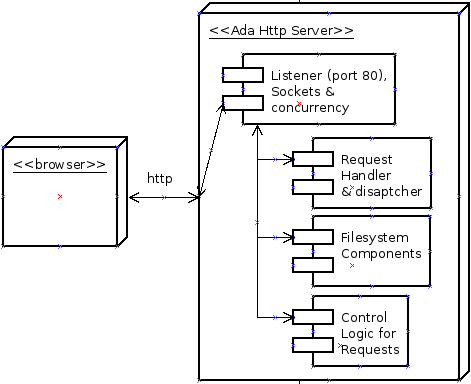
\includegraphics[width=4in]{gfx/deployment.png}
\caption{Deployment Diagram}
\label{fig:deployment}
\end{figure}

  \section{Implementation}
This section will deal with the more technical aspects of this case study. From now on we will list topics that have to do with the implementation of the simple Http server.

\subsection{Defining the required GNAT Project File Specification}
The specifications list the following requirements for the directory structures: 
\begin{table}
\begin{center}
\begin{tabular}{|c|l|}
\hline
src & The directory to contain the sources \\ \hline
obj & The directory to contain the compiler output \\ \hline
bin & The directory to contain the binaries \\ \hline
obj/debug & \parbox{10cm}{The non-optimized compiled binaries with debug info are stored here. You can notice this in the GPR file, where the `-g' flag is given to the compiler.} \\ \hline
obj/release &  \parbox{10cm}{The optimized compiled binaries without debug information. You  can notice this in the GPR file, where the `O2' flag is given to the compiler.} \\ \hline
tests & The directory to contain the tests \\ \hline
\end{tabular}\end{center}
\caption{Directory Structure Specification for GPR File}
\end{table}
\subsubsection{GNAT Project File}
Here is the project file we will be using.
\lstinputlisting[caption=GNAT Project File,language=Ada]{../axios/axios.gpr}
Notice that some of the flags for the compiler in both release, and debug modes are the same flags used for GNU C++ compiler. We explain each section with a little more detail.

\paragraph{Directory Structure}The directory structure is as outlined on the previously demonstrated table. We see these defined in the GPR file by the names of \textbf{Source\_Dirs}, \textbf{Exec\_Dir}. Because of the definition of the Object file directories for a debug and release version, we also get the ``obj/release'' and ``obj/debug'' directories, as previously required. A Simple hello world application would yield the following structure, for example: 

\lstinputlisting[caption=Directory Structure,language=ruby]{src/misc/dir-struct.txt}

\paragraph{Flags} There are many flags that can be set for the compilation and linking process. The manual covers a lot of them, but the ones used are explained.

\subparagraph{Builder} Notice the "package Builder is ..." line. We define the flags that should be used by the builder (gnatmake), when invoked.

\subparagraph{Executable} This is to specify the output name of the binary once the whole project is compiled.

\subparagraph{Compiler} Notice the "package Compiler is ..." line. This contains the flags for the actual compiler. We have two flags `-g', and `-O2' that the seasoned GNU C++ compiler user would recognize instantly. The `-g' flag would be used to produce non-optimized binaries in order to contain extra information when debugging. 
The `-O2' is for optimization, and that is the reason why it is in the release case. We define a Mode\_Type which can either be one of the two literals `debug', and `release' in order to achieve this. 

\subsection{Components}
We now describe the components of the project. 

\subsubsection{Listener}
\paragraph{Specification} Here is the code listing for the listener specification
\lstinputlisting[language=Ada,caption={Simple Listener Specification}]{../axios/src/listener.adb}

\paragraph{Implementation} Here is the code listing for the listener implementation
\lstinputlisting[language=Ada,caption={Simple Listener Body}]{../axios/src/listener.adb}

\section{Testing}
Testing is achieved by using \textbf{AUnit} in order to do unit testing. 


\bibliography{mybib}{}
\bibliographystyle{plain}	
\end{document}
